\title{PS4 Solutions}

%TEMPLATE HEADER
%This is the homework solution template
\documentclass[11pt]{article}

%AMS-TeX packages
\usepackage{amssymb, amsmath, amsthm} 
\usepackage[margin=.75in]{geometry}
\usepackage{graphicx}
\usepackage{caption}
\usepackage{subcaption}
\usepackage{bm} % bold math
\usepackage{listings}
\usepackage{color} %red, green, blue, yellow, cyan, magenta, black, white
\definecolor{mygreen}{RGB}{28,172,0} % color values Red, Green, Blue
\definecolor{mylilas}{RGB}{170,55,241}

%Redefining sections as problems
\makeatletter
\newenvironment{problem}{\@startsection
       {section}
       {1}
       {-.2em}
       {-3.5ex plus -1ex minus -.2ex}
       {0.2ex plus .2ex}
       {\pagebreak[3]%forces pagebreak when space is small; use \eject for better results
       \Large\sc\noindent{Problem }}\\}
\makeatother

%Fancy-header package to modify header/page numbering 
\usepackage{fancyhdr}
\pagestyle{fancy}
\lhead{\textbf{Ge/ESE 118}} %name of the course
\chead{\textbf{}} %topic of the homework set
\rhead{\textbf{Solution 4}} %number of the homework set
\lfoot{}
\cfoot{}
\rfoot{\thepage}

%Include frequently used commands used for equations
%Fractions
\newcommand\fr[2]{\frac{#1}{#2}} %Regular fraction

%Braces, Brackets, Parentheses, etc.
\newcommand\brcs[1]{\{#1\}} %Braces
\newcommand\brckts[1]{\left[#1\right]} %Brackets
\newcommand\lr[1]{\left(#1\right)} %Parentheses
\newcommand\abs[1]{\Big\lvert#1\Big\rvert} %Absolute value
\newcommand\ltwo[1]{\lVert#1\rVert_2} %L2-norm
\newcommand\linf[1]{\lVert#1\rVert_\infty} %L2-norm

%Linear algebra
\newcommand\tr[1]{\text{tr}\left( \mathbf{#1}\right)} %Trace
\renewcommand\det[1]{\text{det}\left( \mathbf{#1}\right)} %Determinant

%Trigonometric & special functions
\newcommand\sinb[1]{\, \sin\left(#1\right)} %Sine with parentheses: sin(x)
\newcommand\cosb[1]{\, \cos\left(#1\right)} %Cosine with parentheses: cos(x)
\newcommand\tanb[1]{\, \tan\left(#1\right)} %Tangent with parentheses: tan(x)
\newcommand\cotb[1]{\, \cot\left(#1\right)} %Cotangent with parentheses: cot(x)
\newcommand\sinc[1]{\, \text{sinc}\left(#1\right)} %Sinc function: sinc = sin(x)/x

%Calculus
\renewcommand\d[1]{\, \text{d}#1} %Differential for integrals
\newcommand\der[2]{\frac{\text{d}#1}{\text{d}#2}} %Ordinary derivate first order
\newcommand\dder[2]{\frac{\text{d}^2#1}{\text{d}#2^2}} %Ordinary derivate second order
\newcommand\od[3]{\frac{\text{d}^{#3}#1}{\text{d}#2^{#3}}} %Ordinary derivate any order
\newcommand\pder[2]{\frac{\partial#1}{\partial#2}} %Partial derivate first order
\newcommand\pdder[2]{\frac{\partial^2#1}{\partial#2^2}} %Partial derivate second order
\newcommand\pd[3]{\frac{\partial^{#3}#1}{\partial#2^{#3}}} %Partial derivative any order

%Fourier transform
\newcommand\ft[1]{\hat{#1}} %Fourier coefficient

%Probability theory, Statistics
\newcommand\ex[1]{\mathbb{E}\left[#1\right]} %Expectation
\newcommand\pr[1]{\mathbb{P}\left(#1\right)} %Probability
\newcommand\Var[1]{\text{Var}\left(#1\right)} %Variance
\newcommand\Cov[1]{\text{Cov}\left(#1\right)} %Covariance
\newcommand\one{\mathbf{1}} %Unity

%Miscellaneous 
\renewcommand\mod{\text{mod}} %Modulo

%CONTENTS OF THE HW SET SOLUTION BEGIN HERE
\begin{document}
\lstset{language=Matlab,%
	  %basicstyle=\color{red},
  breaklines=true,%
  morekeywords={matlab2tikz},
  keywordstyle=\color{blue},%
  morekeywords=[2]{1}, keywordstyle=[2]{\color{black}},
  identifierstyle=\color{black},%}
  stringstyle=\color{mylilas},
  commentstyle=\color{mygreen},%
  showstringspaces=false,%without this there will be a symbol in the places where there is a space
  numbers=left,%
  numberstyle={\tiny \color{black}},% size of the numbers
  numbersep=9pt, % this defines how far the numbers are from the text
  emph=[1]{for,end,break},emphstyle=[1]\color{red}, %some words to emphasise
													  %emph=[2]{word1,word2}, emphstyle=[2]{style},    
}


\subsection*{Problem 1 (graded by Dunzhu) 30 points}
\subsubsection*{(a) - 5 points}

Here 
\begin{eqnarray*}
F(m) = \sum_i \frac{ (d_i - g_i(m))^2}{2 \sigma_d ^2}
\end{eqnarray*}

\begin{eqnarray*}
P(m | d) \propto P(d|m) \propto \exp\left( -F(m) \right) \approx \exp\left( 
-F(m_0) - \frac{\partial F}{\partial m}^T (m-m_0) - \frac{1}{2}(m-m_0)^T \frac{\partial^2 F}{\partial m \partial m} (m-m_0) 
\right) 
\end{eqnarray*}
Above equation has the form of a multivariate Gaussian distribution, So the covariance matrix will be
\begin{eqnarray*}
cov(m) = \left( \frac{\partial^2 F}{\partial m \partial m} |_{m=m_0} \right)^{-1} = H^{-1}
\end{eqnarray*}
Note we want to know covariance matrix when $m_0$ is the best least square model. Using hw2's convention, define
\begin{eqnarray*}
\hat{G}_{i,k} = \frac{\partial g_i}{\partial m_k}
\end{eqnarray*}
Now
\begin{eqnarray*}
H \approx \frac{\hat{G}^{T}\hat{G}}{\sigma_d^2}
\end{eqnarray*}


\lstinputlisting{hw4_p1.m}
the output is
\begin{verbatim}
C0 =

    0.3651   -0.8059    0.7507   -1.3922    0.0480
   -0.8059    2.8090   -2.5992    1.9509   -0.0010
    0.7507   -2.5992    2.4548   -1.7962    0.0010
   -1.3922    1.9509   -1.7962    6.5912   -0.2971
    0.0480   -0.0010    0.0010   -0.2971    0.0171


\end{verbatim}

\subsubsection*{(b)- 5 points}
The covariance matrix calculated here will be similar to the Monte Carlo simulation in HW2. They should be more and more similar when $\sigma_d \rightarrow 0$. 

Diagonal element shows the variance of each parameter. For example, we can notice $\sigma_t^2=0.3651$, $\sigma_x^2 = 2.8099 \approx \sigma_y^2 = 2.4548$. $\sigma_z$ is much larger than $\sigma_x$ and $\sigma_y$. 

The off diagonal shows trade off between parameters. 
For example, $\sigma_{xy} = -2.5992$, explains the linear shape of $(x_s,y_s)$in HW2. Also note $\sigma_{zt}=-1.3922$ indicate strong trade off between $z_s$ and $t_s$. 

Note also it's common to change the covariance matrix to correlation matrix. For example, $\rho_{xy} = \sigma_{xy}/(\sigma_x \sigma_y)$. In this case 

\begin{verbatim}
S=diag(sqrt(diag(C0)));
rho = S^(-1)*C0*S^(-1)
rho =
    1.0000   -0.7958    0.7929   -0.8975    0.6065
   -0.7958    1.0000   -0.9898    0.4534   -0.0046
    0.7929   -0.9898    1.0000   -0.4465    0.0047
   -0.8975    0.4534   -0.4465    1.0000   -0.8840
    0.6065   -0.0046    0.0047   -0.8840    1.0000
\end{verbatim}

the correlation matrix shows $\rho_{zv}=-0.8840$, also a strong tradeoff. 

\subsubsection*{(c)- 5 points}
Now
\begin{eqnarray*}
F(m) = \frac{1}{2\sigma^2} (d - G m)^T (d-G m)
\end{eqnarray*}
where $\sigma=40$, and 
\begin{eqnarray*}
G= [ones(length(x),1),  x]\\
m =[m1, m2]^T
\end{eqnarray*}
So the Hessian is
\begin{eqnarray*}
H = \frac{1}{\sigma^2} G^T G
\end{eqnarray*}
and thus
\begin{eqnarray*}
cov(m) = H^{-1} 
\end{eqnarray*}

\begin{verbatim}
G=[ones(length(x),1), x(:)];
sigma=40;
cov0 = inv(G'*G/sigma^2)

cov0 =

       164.83       -3.084
       -3.084      0.11213



\end{verbatim}

\subsubsection*{(d)- 5 points}
Since in this case, we assume uniform prior, then $P(m|d) \propto P(d|m)$. 
The full parameter space calculate the likelihood  $P(d|m)$, while the covariance is calculated from distribution $P(m|d)$.  So the error map in full-parameter-space in HW2, forms an ellipsoid, whose axis length and rotation angle is all determined by this covariance matrix. For example, the box containing the error ellipsoid has height/width ratio about $(500-100)/(2- (-8)) \approx 4/1 $, which is similar to $\sqrt{164.83/0.11213}$. The off diagnoal is negative, explains the negative slope in HW2. 

\subsubsection*{(e)- 5 points}

First calculate the misfit $F(m)$ for different models. Then the likelihood $P(d|m_1,m_2)$ can be calculated using $\exp(-F(m))$. Then the $P(m_1,m_2|d)$ follows from Bayesian law and uniform prior. Then we can integrate $P(m_1,m_2|d)$ to get the marginal pdf. Finally, we need to make sure the result is normallized properly (it's indeed a pdf, whose integration is 1). 
 
\begin{eqnarray*}
P(m_1, m_2 | d) \propto  \exp( -F(m) )  \\
P(m_1, m_2 | d) = \frac{\exp{F(m)}}{\int dm_1 \int dm_2 \exp{F(m)}}
\end{eqnarray*}

and marginal
\begin{eqnarray*}
P(m_1| d) = \int dm_2 \left( \frac{\exp{F(m)}}{\int dm_1 \int dm_2 \exp{F(m)}} \right ) \\
P(m_2| d) = \int dm_1 \left( \frac{\exp{F(m)}}{\int dm_1 \int dm_2 \exp{F(m)}} \right ) \\
\end{eqnarray*}

We can use summation to approximate the integration. 

\begin{verbatim}
minmis = min(misfit2(:));  % minimum misfit
Pd_m = exp(- (misfit2-minmis) / (2*sigma^2)  ); % likelihood, without normalize 

Pd_m = Pd_m / sum(Pd_m(:)); 
Pm1_d = sum(Pd_m,2)/(m1(2)-m1(1));   %% now int (Pm1_d) dm1 = 1
Pm2_d = sum(Pd_m,1)/(m2(2)-m2(1));

subplot(121);
plot(m1,Pm1_d);
subplot(122);
plot(m2,Pm2_d);
\end{verbatim}
\begin{figure}
\begin{center}
  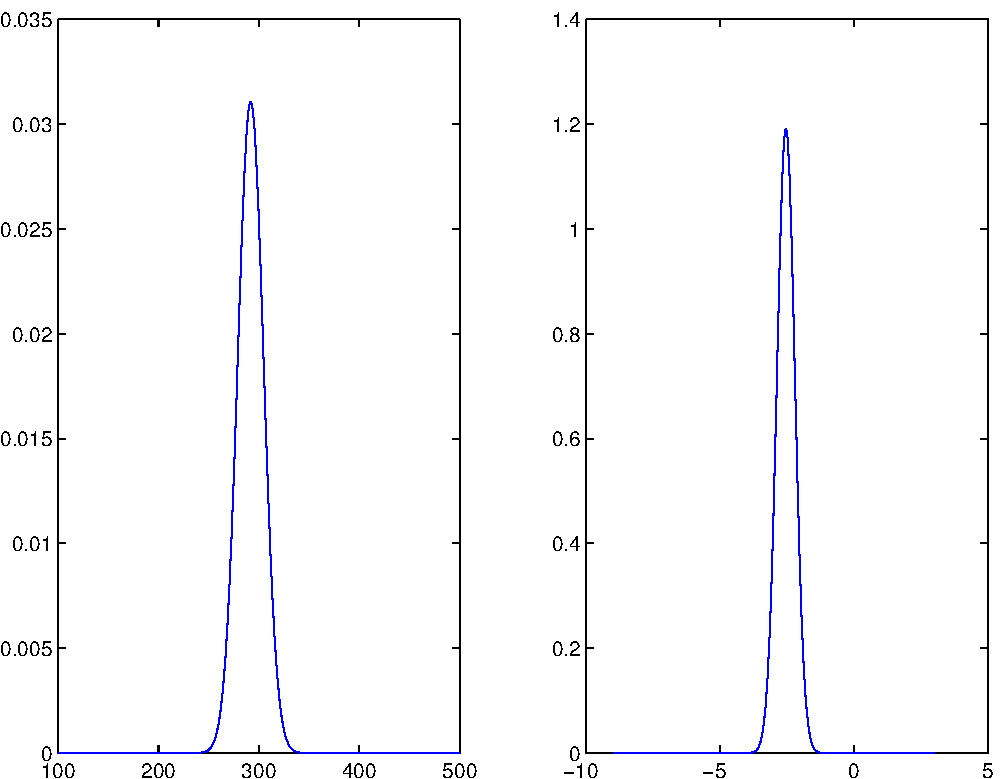
\includegraphics[width=12cm]{p1e.pdf}
  \caption{(e): Marginal pdf for $m_1$ and $m_2$. }
  \end{center}
\end{figure}

\subsubsection*{(f)- 5 points}
\begin{eqnarray*}
\sigma_{m1}^2 = E[m_1^2] - (E[m_1])^2 = \int p(m_1|d) m_1^2 dm_1 - \left(  \int p(m_1|d) m_1 dm_1  \right)
\end{eqnarray*}

\begin{verbatim}
Em1 =  sum(Pm1_d(:) .* m1(:) * (m1(2)-m1(1)) ) ;
Em1m1 = sum(Pm1_d(:) .* m1(:).^2 * (m1(2)-m1(1)) ) ;
Em2 =  sum(Pm2_d(:) .* m2(:) * (m2(2)-m2(1)) ) ;
Em2m2 = sum(Pm2_d(:) .* m2(:).^2 * (m2(2)-m2(1)) ) ;

sigma_m1 = sqrt(Em1m1-Em1*Em1)
sigma_m2 = sqrt(Em2m2-Em2*Em2)

sigma_m1 =

       12.838


sigma_m2 =

      0.33485

\end{verbatim}

Note that $\sigma_{m1}$, $\sigma_{m2}$ is equal to square root of the diagnoal of the covirance matrix calculated in (c). 


\clearpage
\subsection*{Problem 2 (graded by Toby) - 15 points}

\subsubsection*{(a)}
The posterior probability is given by
\begin{equation}
p(\mu|\v{x}) \propto \left( \sum_{k=1}^N (x_k - \mu)^2 \right)^{-\frac{N-1}{2}} =\exp \left( -\frac{N-1}{2} \ln \left[ \sum_{k=1}^N (x_k - \mu)^2 \right] \right).
\end{equation}
Minima of $F$ maximize the probability density function. We have that
\begin{subequations}
\begin{align}
F(\mu) &= \frac{N-1}{2} \ln \left( \sum_{k=1}^N (x_k-\mu)^2 \right), \\
\frac{\partial F}{\partial \mu} &= -(N-1) \frac{\sum_{k=1}^N(x_k - \mu)}{\sum_{k=1}^N(x_k - \mu)^2}\\
\frac{\partial^2 F}{\partial \mu^2} &= (N-1) \frac{N\sum_{k=1}^N(x_k - \mu)^2+2\sum_{k=1}^N(x_k - \mu)}{\left(\sum_{k=1}^N(x_k - \mu)^2\right)^2}.
\end{align}
\end{subequations}
Because $\exp$ and $\ln$ are monotonic functions, we therefore need to find the minimum of the sum of the equared error (least-squares)
\begin{equation}
\sum_{k=1}^N (x_k - \mu)^2 = 0.
\end{equation}
Taking the derivative with respct to $\mu$ and setting it to zero yields the minimum $\mu_0$
\begin{equation}
\mu_0 = \frac{1}{N} \sum_{k=1}^N x_k, 
\end{equation}
which is the sample mean of the data. For the standard deviation $\sigma_\mu$ we expand $F$ to second order and insert $\mu_0$, i.e., 
\begin{equation}
p(\mu|\v{x}) \propto e^{-F(\mu)} \approx e^{-F(\mu_0) - \frac{1}{2}F''(\mu_0)(\mu - \mu_0)^2}, 
\end{equation}
For the second derivate at the best fit solution we have
\begin{equation}
\frac{\partial^2 F}{\partial \mu^2} = \frac{N(N-1)}{\sum_{k=1}^N(x_k - \mu)^2}.
\end{equation}
The standard deviation $\sigma_\mu$ then amounts to
\begin{equation}
\sigma_\mu = \frac{1}{F''(\mu_0)^{1/2}} = \frac{S}{\sqrt{N}}, 
\end{equation}
where 
\begin{equation}
S = \sqrt{\frac{1}{N-1} \sum_{k=1}^N (x_k - \mu_0)^2 }
\end{equation}
is the sample variance of the data.

\subsection*{(b)}
\subsubsection*{Formal general proof}
We prove that an orthogonal matrix $\mathbf{Q}$ does not impact the norm of a vector $\v{x}$. Then $\mathbf{Q}$ is called an isometry. If the length of an arbitrary vector is preserved, $\mathbf{Q}$ must be a rotation matrix, because only rotations leave the length of  vector unchanges. To prove this, we use the $\mathcal{L}_2$-norm of an arbitrary vector $x$ and the fact that for orthogonal matrices, we have $\v{Q}^{-1} = \v{Q}^T$. We can then write
\begin{equation}
\ltwo{\v{x}} = \v{x}^T\v{x} = \v{x}^T \mathbf{1} \v{x} = \v{x}^T\v{Q}^{-1}\v{Q}\v{x} = \v{x}^T\v{Q}^T\v{Q}\v{x} = (\v{Q}\v{x})^T(\v{Q}\v{x}) = \ltwo{\v{Q}\v{x}}.
\end{equation}
Since the left hand side and the right hand side are equal, we have shown that the lengths are equal and unchanged under orthogonal transformations.

\subsubsection*{Simple proof in 2D}
In two dimensions, we have that $\v{Q} = (\v{e}_1\,\, \v{e}_2)$, where $\v{e}_i$ are the column vectors of $\v{Q}$. They are orthonormal. Now, operating $\v{Q}$ on the column vector $\v{x} = (x_1,\, x_2)^T$ gives
\begin{equation}
\v{x}' = \v{Q}\v{x} = x_1\v{e}_1 + x_2\v{e}_2, 
\end{equation}
which is the representation of the vector $\v{x}'$ in the eigenbasis of $\v{H}$. Because the $\v{e}_i$ have length 1, the vector $\v{x}'$ has length $\sqrt{x_1^2 + x_2^2}$. But this is the length of $\v{x}$ as well. So $\v{x}$ and $\v{x}'$ are of the same magnitude. Formally, we have
\begin{equation}
\ltwo{\v{x}'} = \v{x}'^T\v{x}' = x_1^2\v{e}_1^T\v{e}_1 + x_2^2\v{e}_2^T\v{e}_2 + 2x_1x_2\v{e}_1^T\v{e}_2 = x_1^2 + x_2^2 = \v{x}^T\v{x} = \ltwo{\v{x}}.
\end{equation}
This is exactly (!) the same logic as in the general proof but applied explicitly for the two-dimensional problem.

\subsubsection*{Simple explanation}
Because $\v{x}^T \v{H} \v{x} = \text{const}.$ defines an ellipse when $\v{H}$ is symmetric, where the eigenvectors of $\v{H}$ define the principle axes of the ellipse, we can think of $\v{Q} \v{x}$ as a rotation into a coordinate system aligned with these principle axes. This can be seen from $\v{x}'^T \v{\Lambda} \v{x}' = \text{const}$, which also defines an ellipse, but with the principle axes aligned with the coordinate axes (since $\v{\Lambda}$ is diagonal).

\subsubsection*{(c)}
We need to show that $\sigma_x^2 = \frac{B}{AB-C^2}$. We are deadling with an integral of the form
\begin{subequations}
\begin{align}
\sigma_x^2 &= \frac{\int dx dy \, x^2 \exp\left( -\frac{1}{2}\v{x}^T \v{A} \v{x}  \right)}{\int dx dy \, \exp\left( -\frac{1}{2}\v{x}^T \v{A} \v{x}  \right)}\\
&= \frac{\int \d{x} \d{y} \, x^2 \exp\left( -\frac{1}{2}(Ax^2 + 2Cxy +By^2)  \right)}{\int \d{x} \d{y} \, \exp\left( -\frac{1}{2}(Ax^2 + 2Cxy +By^2)  \right)}\\
&= \frac{\int \d{x} \d{y} \, x^2 \exp\left( -\frac{1}{2}(A-C^2/B)x^2 -\frac{1}{2}B(y + Cx/B)^2  \right)}{\int \d{x} \d{y} \, \exp\left( -\frac{1}{2}(A-C^2/B)x^2 -\frac{1}{2}B(y + Cx/B)^2  \right)}\\
&= \frac{\int \d{x} \, x^2 \exp\left( -\frac{1}{2}(A-C^2/B)x^2 \right)}{\int \d{x} \, \exp\left( -\frac{1}{2}(A-C^2/B)x^2 \right)}
\end{align}
\end{subequations}
If we set $\sigma^2 = 1/(A-C^2/B)$, we arrive at
\begin{equation}
\sigma_x^2 = \frac{\int \d{x} \, x^2 \exp\left( -\frac{1}{2}x^2/\sigma^2 \right)}{\int \d{x} \, \exp\left( -\frac{1}{2}x^2/\sigma^2 \right)}
\end{equation}, 
which as we have seen in previous homework sets and solutions implies
\begin{equation}
\sigma_x^2 = \langle x^2\rangle = \sigma^2 = \frac{1}{A-\frac{C^2}{B}} = \frac{B}{AB-C^2}.
\end{equation}
The hint was used in step 3. In step 4 we integrated out the $y$-dependence because the integration boundaries of $\pm \infty$.

\subsection*{Problem 3 (graded by Stephen) - 35 points}


\subsubsection*{(a) - 5 points}
It is not reasonable to assume that all model parameters have constant priors (-$\infty$ to $\infty$).  We know that $t_s$ should occur before all of the observations (for the signal to be causal, at least to within errors on the data, i.e. $t_s<322$~s) and velocity must be positive (thus $v>0$).  We can leave these priors from $-\infty$ to $322$~s and 0 to $\infty$, respectively, even though we know that there is a physical upper limit (for example $v$ cannot be faster than the speed of light). The prior for $z_s$ should be restricted to positve or negative values, depending on our sign convention for the height coordinate, because the earthquake occured below the surface. Practically, we can leave the priors on $x_s$, $y_s$ as constant priors, but in reality they also would be limited to the size of the earth.

\subsubsection*{(b) - 5 points}
We can incorporate this information as a prior by multiplying our likelihood $P(\{t_k\}|m)$ by a prior for velocity $P\{v\}$.  In this case we will use a Gaussian prior with $\mu = 4.8$ and $\sigma = 0.1$.  Other variables get uniform priors. Our expression will look like:

\begin{eqnarray*}
P\{v\}=e^{-\frac{1}{2}(\frac{v-\mu}{\sigma})^2} \\
P(m|\{t_k\})=P(\{t_k\}|m)P\{v\} \\
P(m|\{t_k\})=e^{-F(m)}e^{-\frac{1}{2}(\frac{v-\mu}{\sigma})^2} \\
P(m|\{t_k\})=e^{-F(m)-\frac{1}{2}(\frac{v-\mu}{\sigma})^2}
\end{eqnarray*}

Note also that the the velocity should be positive. This is only approximately the case for the Gaussian prior, but is not a problem, because the probability for negative velocities is very (!) small.

\subsubsection*{(c.i) - 5 points}
\begin{eqnarray*}
\int_{v_1}^{v_2} {P(v)dv} = \int_{v_1}^{v_2} {\frac{1}{v}dv} = \ln(v_2) - \ln(v_1) \\
\int_{kv_1}^{kv_2} {P(v)dv} = \int_{kv_1}^{kv_2} {\frac{1}{v}dv} = \ln(kv_2) - \ln(kv_1) \\
= \ln(k)+\ln(v_2)-\ln(k)-\ln(v_1) \\
= \ln(v_2) - \ln(v_1)
\end{eqnarray*}

\subsubsection*{(c.ii) - 5 points}
We can again incorporate this information as a prior in our expression for $P(m|\{t_k\})$ by multiplying it times our likelihood (just like in part b).  Our expresssion becomes:

\begin{eqnarray*}
P(m|\{t_k\}) = e^{-F(m)} \frac{1}{v}
\end{eqnarray*}

\subsubsection*{(d) - 5 points}
We want to incorporate both independent pieces of information into our prior.  In this case we can multiply the two priors together.  Our new expression becomes:

\begin{eqnarray*}
P(m|\{t_k\}) =  \frac{1}{v} e^{-F(m)} e^{-\frac{1}{2}(\frac{v-\mu}{\sigma})^2}
\end{eqnarray*}

Let's plot the two priors separately and then together to see which information dominates the result.  Figure 2 is the Gaussian prior.  Figure 3 is the scale independent prior.  Figure 4 is their combination.  We can see that the Gaussian prior is scaled by the scale invariant prior, but still mainly retains it's shape and thus dominates the result.

\begin{figure}
\begin{center}
  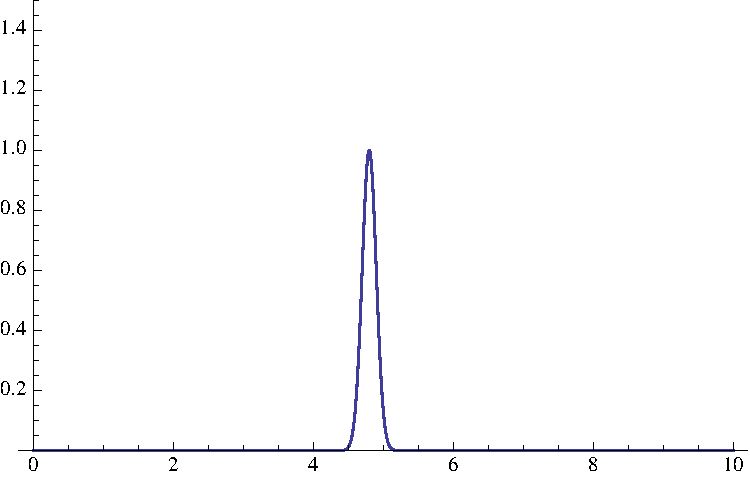
\includegraphics[width=12cm]{ESE118_PS4_P3_Fig1.pdf}
  \caption{Plot of the Gaussian prior for velocity.}
  \end{center}
\end{figure}

\begin{figure}
\begin{center}
  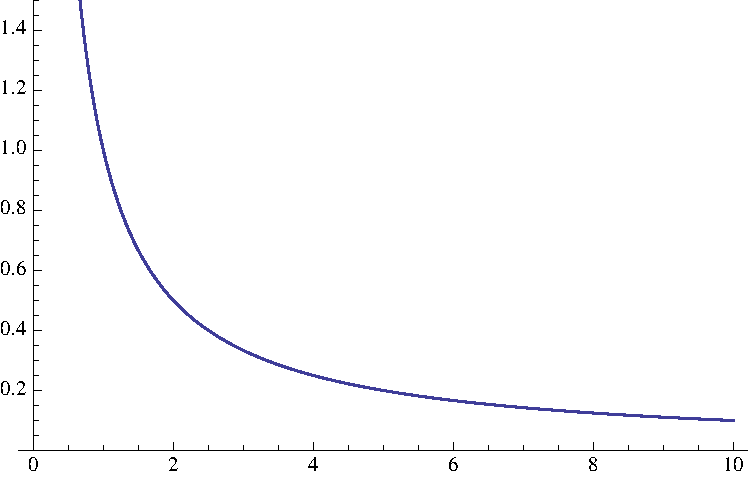
\includegraphics[width=12cm]{ESE118_PS4_P3_Fig2.pdf}
  \caption{Plot of the scale invariant prior for velocity.}
  \end{center}
\end{figure}

\begin{figure}
\begin{center}
  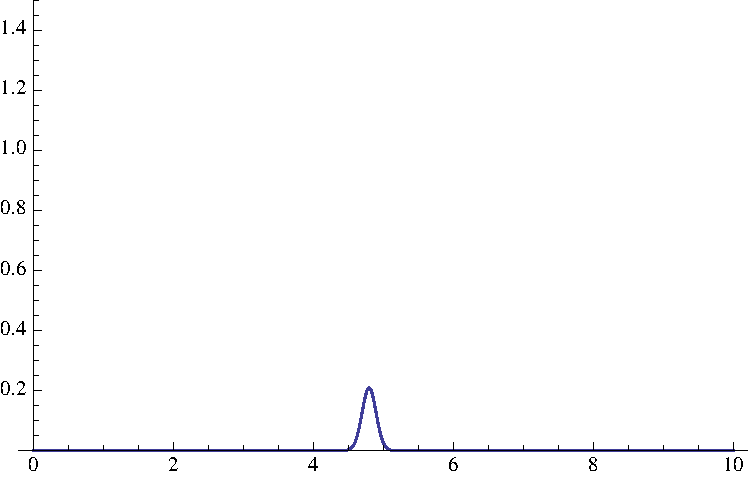
\includegraphics[width=12cm]{ESE118_PS4_P3_Fig3.pdf}
  \caption{Plot of combination of the Gaussian and scale invariant priors for velocity.  Note how the plot is scaled but retains basically the same shape as the pure Gaussian.}
  \end{center}
\end{figure}

\subsubsection*{(e) - 5 points}
It doesn't matter in what order we do things as long as priors for analysis are not biased by our data (and they shouldn't be).  If we did the experiment without talking to our friends, we would have no extra information and would use uniform priors.  If we talk to them first, we use the non-uniform prior we derived in the previous step.


\subsubsection*{(f) - 5 points}
Previous expression: $P(m|\{t_k\}) = e^{-F(m)}$ \\
New expression: $P(m|\{t_k\}) =  \frac{1}{v} e^{-F(m)} e^{-\frac{1}{2}(\frac{v-\mu}{\sigma})^2}$ \\

Previous misfit function: $F(m)$ \\
To find the new misfit function we will need to manipulate our expression to get everything into a single exponential.  Let's start with the $\frac{1}{v}$ part:

\begin{eqnarray*}
\frac{1}{v} = e^{(\ln(\frac{1}{v})} = e^{-\ln(v)} \\
P(m|\{t_k\}) = e^{-\ln(v)} e^{-F(m)} e^{-\frac{1}{2}(\frac{v-\mu}{\sigma})^2} \\
\end{eqnarray*}

New misfit function: $F(m) + \ln(v) + \frac{1}{2}(\frac{v-4.8}{0.1})^2$ \\

We only need to make a couple simple changes to our code from HW2.  Instead of just using the L2 norm as our error function, we now need to add our extra two terms to our misfit function.  We also need to slightly change our $\gamma$ and our Hessian.  Our old Hessians do not take into account the given standard deviation of the data: $\sigma=0.01$.  We can take this into account by doing a simple modification on them:

\begin{eqnarray*}
H_{new} = \frac{H_{old}}{0.01^2} \\
\gamma_{new} = \frac{\gamma_{old}}{0.01^2}
\end{eqnarray*}

We will add a term to the last entries of $\gamma$ and the Hessian to account for the new priors on $v_s$.

Add the first derivative of our new part of the misfit to $\gamma$:

\begin{eqnarray*}
\frac{dF}{dv} = \frac{1}{v} + \frac{v-\mu}{\sigma^2}
\end{eqnarray*}

And the second derivative to the last entry of the Hessian:

\begin{eqnarray*}
\frac{d^2F}{dv^2} = \frac{-1}{v^2} + \frac{1}{\sigma^2}
\end{eqnarray*}



Here is the full code:
\begin{verbatim}
function hw4p3()
rng(0); % this generate determined random variable
xi=[0 10 15 6 -7 3]';
yi=[0 0 6 13 10 7]';
zi=[0 0 0 0 0 0]';
ti=[322.418 321.031 321.228 323.093 324.415 322.706]';

sig = 0.1;
mu = 4.8;

M0=do_one_ti(xi,yi,zi,ti);
ti_0=predict(xi,yi,zi,M0);

function M=do_one_ti(xi,yi,zi,ti)

M=[300 20 -10 10 2]'; % initial guess
for step = 1:10
    M(5);
    grad=zeros(5,1);
    hess=zeros(5,5);   
    for i=1:length(xi)
        [tmp_grad, tmp_hess]=get_grad_hessian(xi(i),yi(i),zi(i),ti(i),M);    
        grad = grad + tmp_grad;
        hess = hess + tmp_hess;   
    end
    
    %adjust the final values of gamma and the Hessian to account for the
    %velocity priors
    grad(end) = grad(end) + 1/(M(5)) + (M(5)-4.8)/(0.1)^2;
    hess(end,end) = hess(end,end) + 1/0.1^2 - 1/M(5).^2;
       
    err(step) = (norm(predict(xi,yi,zi,M)-ti)^2);   
  %  if(step > 1 && err(step) > err(step-1))
  %      break;
  %  end
	M = M- inv(hess)*grad;
end
M
plot(err);

function [grad,hess] = get_grad_hessian(xi,yi,zi,ti,M)
ts=M(1); xs=M(2); ys=M(3); zs=M(4); v=M(5);
R=sqrt((xs-xi)^2 + (ys-yi)^2 + (zs-zi)^2);
nx=(xs-xi)/R;
ny=(ys-yi)/R;
nz=(zs-zi)/R;
e=(ts+R/v-ti);

sig = 0.1;

grad = e*[1 nx/v ny/v nz/v -R/v^2]';
sen = [1 nx/v ny/v nz/v -R/v^2]';
hess = sen*sen'; % approximate hess

%need to add ajustment for sigma given for the data
hess = hess/0.01^2;
grad = grad/0.01^2;

%hess(end,end) = hess(end,end) + 1/sig^2 - 1/v^2;

function r=predict(xi,yi,zi,M)

ts=M(1); xs=M(2); ys=M(3); zs=M(4); v=M(5);
r=xi*0;
for i=1:length(xi)
    R=sqrt((xs-xi(i))^2 + (ys-yi(i))^2 + (zs-zi(i))^2);
    r(i)=(ts+R/v);
end
\end{verbatim}

Our best fit solution is now:
\begin{eqnarray*}
  m & = & 
  \left(
  \begin{array}{c}
  313.9738 \\
   30.9907 \\
  -17.7781 \\
   21.7237 \\
    4.9581 \\
  \end{array}
  \right)
  \end{eqnarray*}
  
Our old best fit solution:

\begin{eqnarray*}
  m & = & 
  \left(
  \begin{array}{c}
      315.147372215551 \\
          30.3124982007349 \\
         -17.1481612373344 \\
          15.9867180697526 \\
          5.26992730665649 
  \end{array}
  \right) 
\end{eqnarray*}

We can see that the addition of these priors did change our solution for some parameters a small amount (mostly a change in the best fit for z is observed).  As we would expect, the solution for v has been pushed closer to 4.8 (given our Gaussian prior around this value) and the other parameters have adjusted accordingly.

\end{document}

























